\documentclass{beamer}
\usepackage{isolatin1}
\usepackage{latexsym}

\usepackage{listings}
\lstset{language=XML,showspaces=false,showtabs=false}

\usepackage[german]{babel}

\usetheme{Berlin}
\mode<presentation>

\title{Integration von RSS mit verteiltem Publish/Subscribe}
\author{Friedemann Zintel}

\begin{document}
\bibliographystyle{ieeetr}

\begin{frame}

  \titlepage

\end{frame}

\section*{Outline}
\begin{frame}

  \tableofcontents

\end{frame}

\section{Einleitung}

\begin{frame}

  \begin{itemize}
    \item Verteilung von Informationen �ber das Internet gewinnt immer mehr an Bedeutung.
    \item Verteilungskonzept: Publish/Subscribe (Pub/Sub)
    \item RSS: Pub/Sub-System, jedoch nicht im herk�mmlichen Sinne
    \item RSS: von viele Anbietern unterst�tzt (beliebt: BLogs)
  \end{itemize}

\end{frame}

\section{�berblick}

\subsection{Publish/Subscribe}
\begin{frame}
  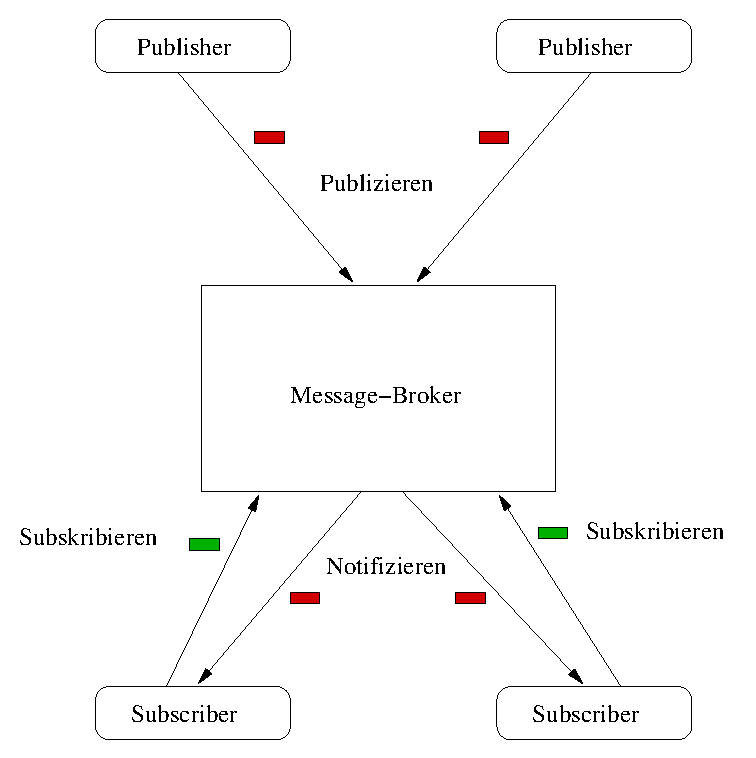
\includegraphics[bb=-50 0 200 350,scale=0.6]{PubSub}
\end{frame}

\subsection{RSS}
\begin{frame}

  \frametitle{RSS: Really Simple Syndication}
  \begin{itemize}
    \item RSS-Feed dient zur Kurzbeschreibung von Web-News
    \item XML-basiert
    \item Erreichbar durch Link auf Anbieterseite
  \end{itemize}
  \nocite{LiuVenSirer:2005:MeasureRSSPubSub}

\end{frame}

\begin{frame}[fragile,allowframebreaks]
  \frametitle{Beispiel: RSS-Feed}
  \tiny
  \begin{lstlisting}
<?xml version="1.0" encoding="iso-8859-1"?>
<!DOCTYPE rss PUBLIC "-//Netscape Communications//DTD RSS 0.91//EN"
  "http://my.netscape.com/publish/formats/rss-0.91.dtd"> 

<rss version="0.91">

<channel>

 <title>SPIEGEL ONLINE</title>
 <link>http://www.spiegel.de</link>
 <description>Schneller wissen, was wichtig ist</description>
 <language>de</language>

 <image>
  <title>SPIEGEL ONLINE</title>
  <url>http://www.spiegel.de/static/sys/logo_120x61.gif</url>
  <link>http://www.spiegel.de</link>
 </image>
  \end{lstlisting}
  \begin{lstlisting}
 <item>
  <title>Bagdad Sniper:  Der Mann, der Juba &#252;berlebte</title>
  <link>http://www.spiegel.de/panorama/0,1518,394137,00.html</link>
 </item>

 <item>
  <title>Infineon:  Vorstand streitet &#252;ber Speichersparte</title>
  <link>http://www.spiegel.de/wirtschaft/0,1518,394143,00.html</link>
 </item>

 <item>
  <title>Biathlon:  Glagow l&#228;uft Olympiasiegerin davon</title>
  <link>http://www.spiegel.de/sport/wintersport/0,1518,394138,00.html</link>
 </item>

 </channel>
 </rss>
  \end{lstlisting}
  Quelle: www.heise.de
\end{frame}

\section{Motivation}
\begin{frame}

  \frametitle{Anwendersicht: Was man gerne h�tte ...}
  \begin{itemize}
    \item Automatische Benachrichtigung �ber Feed-Updates
    \item Aktualit�t der Feeds
    \item Definition von Filtern auf h�herer Ebene: zur \dots
      \begin{list}{}{}
        \item \dots individuellen Vorselektion der News
	\item \dots anbieter�bergreifenden Zusammenstellung neuer Feeds
      \end{list}
  \end{itemize}

\end{frame}

\begin{frame}

  \frametitle{Stand der Dinge}
  \begin{itemize}
    \item RSS: Kein Pub/Sub im herk�mmlichen Sinne $\rightarrow$ Client/Server
    \item Feeds m�ssen von Anwendersoftware erfragt werden (Polling)
    \item Vordefinierte Channel $\rightarrow$ thematische Zuordnung auf Publisherseite
    \item Definition von Filtern nur auf Anwenderseite m�glich
  \end{itemize}

  \pause
  Probleme:
  \begin{itemize}
    \item Polling:
      \begin{list}{$\longrightarrow$}{}
        \item Gro�er Datenverkehr im Netz
	\item Hohe serverseitige Last
      \end{list}
    \item Filterdefinition nur beim Anwender:
      \begin{list}{$\longrightarrow$}{}
        \item alle Feeds m�ssen gedownloaded werden
      \end{list}
  \end{itemize}
  \nocite{Hicks:2004:RSSBandwith}
  
\end{frame}

\begin{frame}

  \frametitle{Ziel}
  \begin{itemize}
    \item Verteilung der RSS-Feeds mittels herk�mmlichem Pub/Sub $\Longrightarrow$ Notifikation der Subscriber
    \item Erm�glichung der subscriberseitigen Definition von Filtern
    \item Reduzierung des Datenverkehrs durch RSS-Polling
    \item Entlastung der RSS-Server
  \end{itemize}

\end{frame}

\section{Realisierung}
\begin{frame}
  \frametitle{Konstruktion eines Overlay-Broker-Netzwerkes}
\end{frame}

\section{Literatur}
\begin{frame}[allowframebreaks]
  \bibliography{../bibdatabase}
\end{frame}

\end{document}
